\let\negmedspace\undefined
\let\negthickspace\undefined
\documentclass[journal]{IEEEtran}
\usepackage[a5paper, margin=10mm, onecolumn]{geometry}
\usepackage{lmodern} % Ensure lmodern is loaded for pdflatex
\usepackage{tfrupee} % Include tfrupee package

\setlength{\headheight}{1cm} % Set the height of the header box
\setlength{\headsep}{0mm}     % Set the distance between the header box and the top of the text

\usepackage{gvv-book}
\usepackage{gvv}
\usepackage{cite}
\usepackage{amsmath,amssymb,amsfonts,amsthm}
\usepackage{algorithmic}
\usepackage{graphicx}
\usepackage{textcomp}
\usepackage{xcolor}
\usepackage{txfonts}
\usepackage{listings}
\usepackage{enumitem}
\usepackage{mathtools}
\usepackage{gensymb}
\usepackage{comment}
\usepackage[breaklinks=true]{hyperref}
\usepackage{tkz-euclide} 
\usepackage{listings}                                      
\def\inputGnumericTable{}                                 
\usepackage[latin1]{inputenc}                                
\usepackage{color}                                            
\usepackage{array}                                            
\usepackage{longtable}
\usepackage{multicol}
\usepackage{calc}                                             
\usepackage{multirow}                                         
\usepackage{hhline}                                           
\usepackage{ifthen}                                           
\usepackage{lscape}
\begin{document}

\bibliographystyle{IEEEtran}
\vspace{3cm}

\title{10.3.2.2.1}
\author{EE24BTECH11006 - Arnav Mahishi}
% \maketitle
% \newpage
% \bigskip
{\let\newpage\relax\maketitle}

\renewcommand{\thefigure}{\theenumi}
\renewcommand{\thetable}{\theenumi}
\setlength{\intextsep}{10pt} % Space between text and floats


\numberwithin{equation}{enumi}
\numberwithin{figure}{enumi}
\renewcommand{\thetable}{\theenumi}


\textbf{Question}:\newline
Find out whether the lines $5x-4y+8=0$ and $7x+6y-9=0$ intersect at a point, parallel or coincident 
\newline
\begin{table}[h!]    
  \centering
  \begin{tabular}[10pt]{ |c| c| c|}
    \hline
    \textbf{input}&\textbf{Description}&\textbf{value}\\
    \hline 
    $a$&Length of semi major axis of ellipse&$3$\\
    \hline
    $b$&Length of semi minor axis of ellipse&$2$\\
    \hline
    $v$&Quadratic form of matrix&$\myvec{b^2&0\\0&a^2}$\\
    \hline 
    $u$&Linear coefficient vector&$0$\\
    \hline 
    $f$&Constant Term&$-(a^2b^2)$\\
    \hline
    $h$&One of the points the line passes through&$\myvec{a\\0}$\\
    \hline
    $m$&Slope of line&$\myvec{\frac{1}{b}\\\frac{-1}{a}}$\\
    \hline
    $n$& number of subintervals we are taking & $1000$\\
    \hline
    $x_0$&$x$ coordinate of first intersection point& $3$\\
    \hline
    $x_n$& $y$ coordinate of second intersection point& $2$\\
    \hline
    \end{tabular}

  \caption{Variables Used}
  \label{tab1.1.2.2}
\end{table}
\newline
\textbf{Theoretical Solution:}\\
Let $a_1$,$b_1$, and $c_1$ and $a_2$,$b_2$, and $c_2$ be the coefficents of $x$,$y$, and $1$ in lines $1$ and $2$ respectively.\\
We get:
\begin{align}
    \frac{a_1}{a_2}=\frac{5}{7}\\
    \frac{b_1}{b_2}=\frac{-2}{3}\\
    \frac{c_1}{c_2}=\frac{-8}{9}\\
    m_1=\frac{-a_1}{b_1}=\frac{5}{4}\\
    m_2=\frac{-a_2}{b_2}=\frac{7}{6}
\end{align}
As all the ratios aren't equal to each other neither are $m_1$ and $m_2$ equal\\
$\therefore$ The lines intersect at a point\\
\textbf{Computational Solution:}\\
The set of linear equations $5x-4y+8=0$ and $7x+6y-9=0$ can be represented by the following equation
\begin{align}
    \myvec{5&-4\\7&6}\myvec{x\\y}=\myvec{-8\\9}
\end{align}
Any non-sigular matrix can be represented as a product of a lower triangular matrix $L$ and an
upper triangular matrix $U$

\begin{align}
    A\vec{x} = LU\vec{x} = \vec{b}
\end{align}
The upper triangular matrix U is found by row reducing A,
\begin{align}
    \myvec{5 & -4 \\ 7 & 6 } \xrightarrow{R_2 -> R_2 - \frac{7}{5}R_1} \myvec{5 & -4 \\ 0 & \frac{58}{5}}  
\end{align}
Let 
\begin{align}
    L = \myvec{1 & 0\\ l_{21} & 1}
\end{align}
$l_{21}$ is the multiplier used to zero $a_{21}$, so $l_{21} = \frac{7}{5}$.\\
\newline
Now,
\begin{align}
    A = \myvec{5 & -4 \\ 7 & 6 } = \myvec{1 & 0 \\ \frac{7}{5} & 1}\myvec{-8\\9}
\end{align}
Now we can get the solution to our problem by the two step process,
\begin{align}
    L\vec{y} = \vec{b}\\
    U\vec{x} = \vec{y}
\end{align}
Using forward substitution to solve the first equation,
\begin{align}
     \myvec{1 & 0 \\ \frac{7}{5} & 1}\myvec{y_1 \\ y_2} &= \myvec{-8\\9}\\
    \implies \myvec{y_1 \\ y_2} &= \myvec{-8 \\ \frac{101}{5}}\\
\end{align}
Now using back-substitution for the second equation,
\begin{align}
     \myvec{5 & -4 \\ 0 & \frac{58}{5}}\myvec{x_1 \\ x_2} &= \myvec{-8 \\ \frac{101}{5}}\\
    \implies\myvec{x_1 \\ x_2} &= \myvec{\frac{-6}{29} \\ \frac{101}{58}}
\end{align}
Thus,
\bein{align}
    \vec{x}= \myvec{\frac{-6}{29} \\ \frac{101}{58}}
\end{align}
$\therefore$ The lines $5x-4y+8=0$ and $7x+6y-9=0$  intersect at $\brak{\frac{6}{29},\frac{101}{58}}$
\begin{figure}[h!]
   \centering
   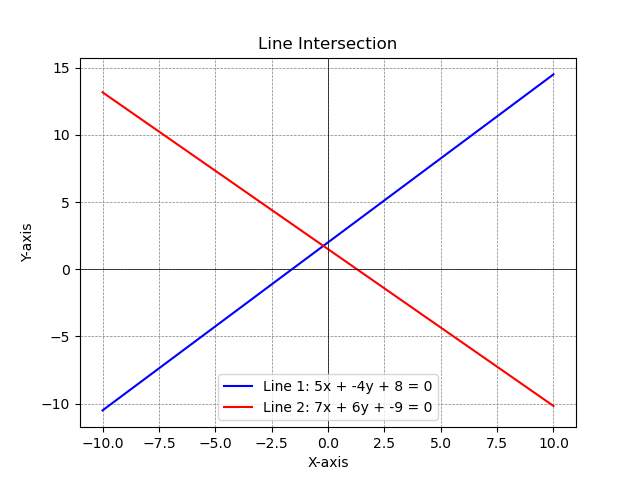
\includegraphics[width=0.7\columnwidth]{figs/fig.png}
    \caption{Solution to set of linear equations}
\end{figure}
\end{document}
